\part{Capitulo 7}

\section{Tipos de Equipos}

\begin{itemize}
    \item Movimiento de Tierras
    \begin{itemize}
        \item Excavadoras (orugas con pala frontal)
        \item Buldozer
        \item Camion Tolva
        \item Retro Excavadora (Pala delantera y brazo atras)
        \item Mononiveladora (Niveladora de caminos)
        \item Motoniveladora (Igual pero con motor)
        \item Cargador Frontal (Pala frontal grande con articulacion en vehiculo y no en las ruedas)
        \item Mototrailla o Trailla (Permite ditribuir tierra)
    \end{itemize}
    \item Compactacion o Nivelacion
    \begin{itemize}
        \item Placa Compactadora (Se usa manualmente)
        \item Rodillo compactador liso (Hay de distintos tamaños)
        \item Rodillo compactador pata de cabra (Se usa para compactar mas profundamente)
        \item Rodillo compactador neumatico (Se usa para compactar asfalto, el que tiene muchas ruedas)
    \end{itemize}
    \item Produccion de Hormigon, existen distintos tipos de maquinas o instalaciones
\end{itemize}

\textbf{Criterios de Seleccion:} Se debe considerar el costo total, lo que comprende la inversion original mas el costo de operacion, costo de reparacion y mantencion del equipo. La suma de todo esto se define como \textbf{INVERSION TOTAL DE UN EQUIPO}

\section{Productividad de Equipos}

De este modo, se busca la productividad optima \textbf{Qp} la cual se basa en la operacion continua de la maquinaria por hora. Se define la productividad normal \textbf{Qv} como Qv incorporando el factor humano (0.85). Ademas si se agrega el factor de direccion del trabajo (fp), se optiene la productividad real \textbf{Qr}

\begin{equation}
    Qr = fp \cdot Qn = fp \cdot fw \cdot Qp = fa \cdot Qp
\end{equation}

\newpage
\section{Costos de Equipos}

Hay que tomar en consideracion costos como depreciacion e inversion inicial:

\begin{figure}[H]
    \centering
    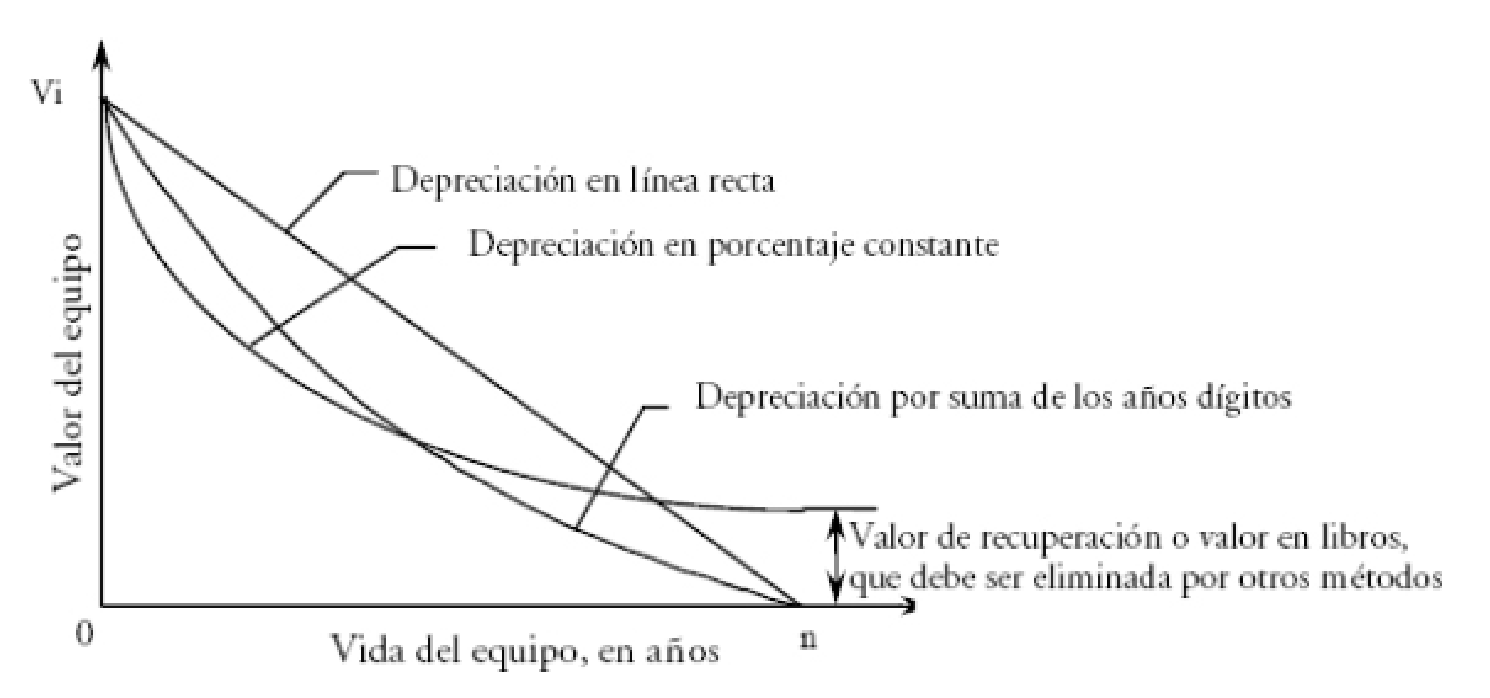
\includegraphics[width=0.8\linewidth]{FOTOS/costo_equipo.png}
    \caption{Costos de Equipos}
    \label{fig:costos}
\end{figure}

\begin{itemize}
    \item Costos de inversion
    \begin{itemize}
        \item Compra 
        \item Internacion
        \item Flete
        \item Seguro de traslado
        \item Intereses
        \item Impuestos
        \item Seguro
        \item Almacenaiento
    \end{itemize}
    \item Costos de operacion
    \begin{itemize}
        \item Operador
        \item Combustible
        \item Lubricacion
        \item mantencion
        \item Reparaciones menores
        \item Neumaticos y Filtros
    \end{itemize}
\end{itemize}

\newpage
\section{Vida Equipo}

De esta forma, la vida de un equipo se define como:

\begin{figure}[H]
    \centering
    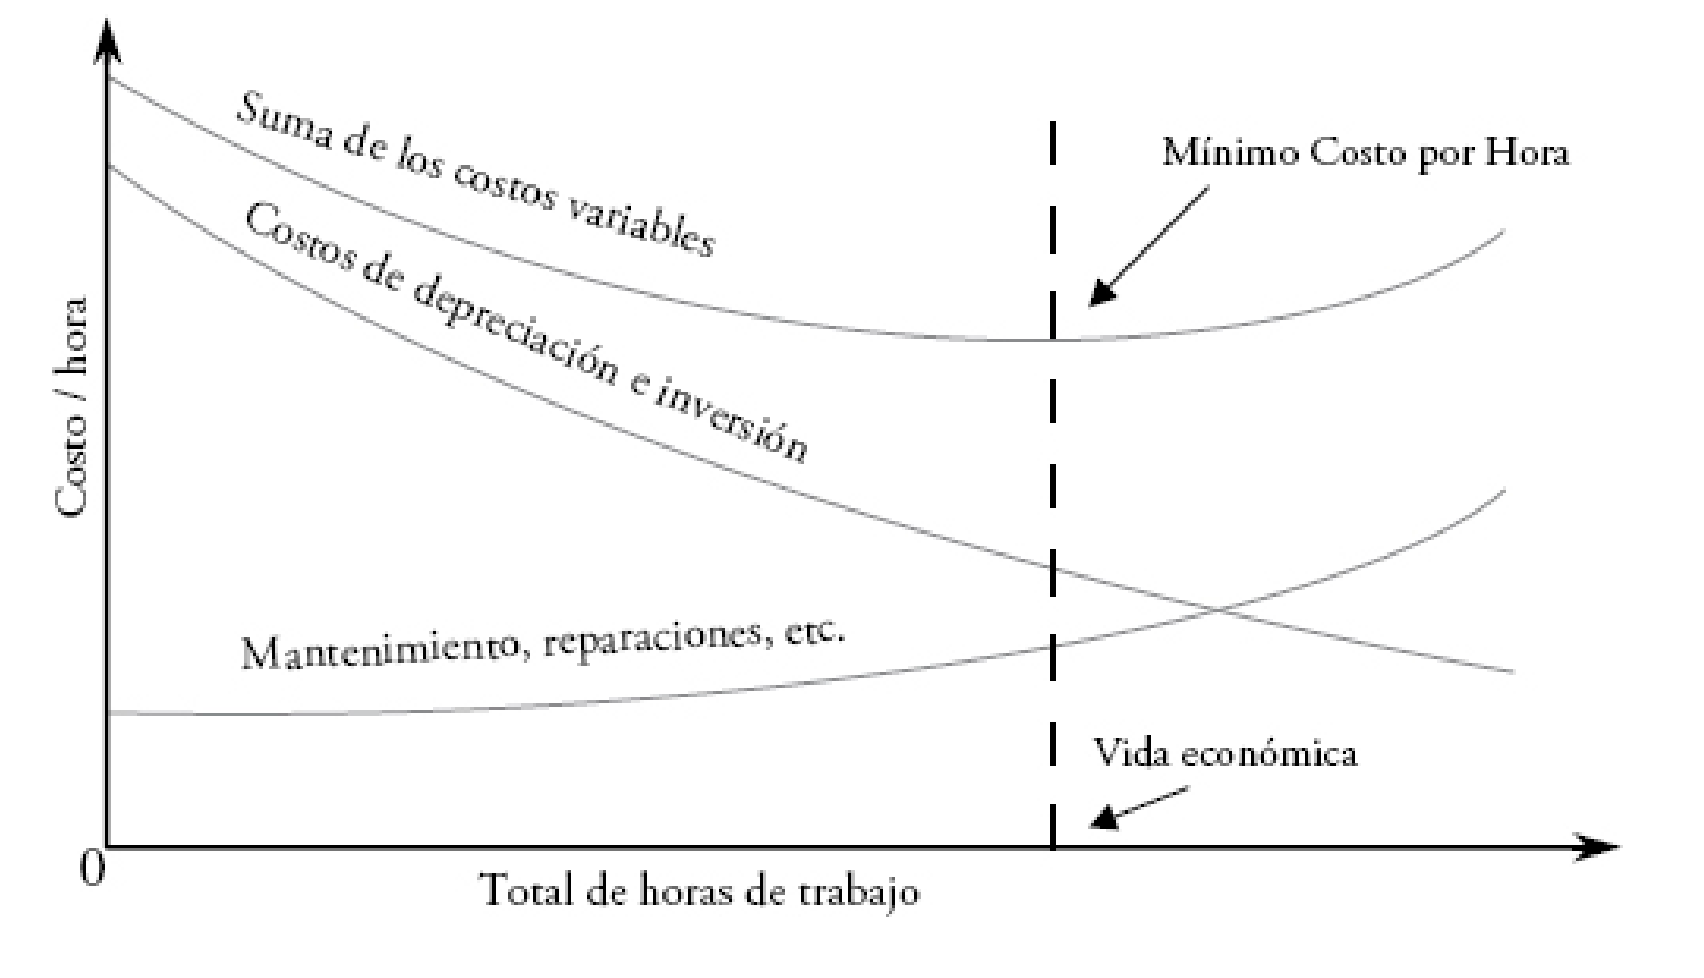
\includegraphics[width=0.8\linewidth]{FOTOS/vida_equipo.png}
    \caption{Vida de un Equipo}
    \label{fig:vida}
\end{figure}